\documentclass[a4paper, 12pt]{extarticle}
\usepackage[english, russian]{babel}
\usepackage[utf8x]{inputenc}
\usepackage{fullpage}
\usepackage{indentfirst} % Первый абзац в разделе тоже с красной строки
\usepackage{cmap} % для кодировки шрифтов в pdf (чтобы не было крокозябры при копировании из pdf )
\usepackage{graphicx} % для вставки картинок
\sloppy % Включение переноса слов в тексте

\usepackage{hyperref} % Для добавления ссылок в тесте

% Настройка цветов для ссылок
\hypersetup{
colorlinks = true,
linkcolor = black,
pagecolor = black,
urlcolor = blue, 
citecolor = black
}

\usepackage[labelfont=bf, labelsep=space]{caption} % Делаем надписи "Рис.1" под рисунками жирными и без двоеточия.

\usepackage[top=20mm, bottom=20mm, left=20mm, right=20mm
, nohead % Убрать расстояние для верхних колонтикулов
%, nofoot % Убрать расстояние для нижних колонтикулов
]
{geometry} % Размер полей у старницы
\setlength{\parindent}{1.25cm} % Размер интервала для абзацев 
\usepackage{setspace}
\onehalfspacing % одинарный интервал

\usepackage{caption} % подписи к рисункам в русской типографской традиции
\DeclareCaptionFormat{GOSTtable}{#2#1\\#3\vspace*{-\baselineskip}}
\DeclareCaptionLabelSeparator{fill}{\hfill}
\DeclareCaptionLabelFormat{fullparents}{\bothIfFirst{#1}{~}#2}
\captionsetup[table]{
     format=GOSTtable,
     %font={footnotesize},
     labelformat=fullparents,
     labelsep=fill,
     labelfont=normal,
     textfont=bf,
     justification=centering,
     singlelinecheck=false
     }

\begin{document}
\section*{Маршрут до места проведения посвята}
\subsection*{Общий вид}
\par Маршрут проложет от Красной площади до места проведения посвята. Сам маршрут Вы можете видеть на рисунке~\ref{ris:generalRoute}. Протяженность маршрута около 20 км, время без пробок 39 минут. Дорога за городом столь убога, что 40 минут светит только внедорожнику. Рассчитывайте время с запасом.

\par Если кто-то хочет самостоятельно построить себе маршрут, то вот примерные координаты для Яндекса 57.541585, 39.700436. В приципе эти же коордитнаты работает на картах от Google. Более того и Google есть StreetView практически на весь маршрут движения.
\begin{figure}[h]
	\center{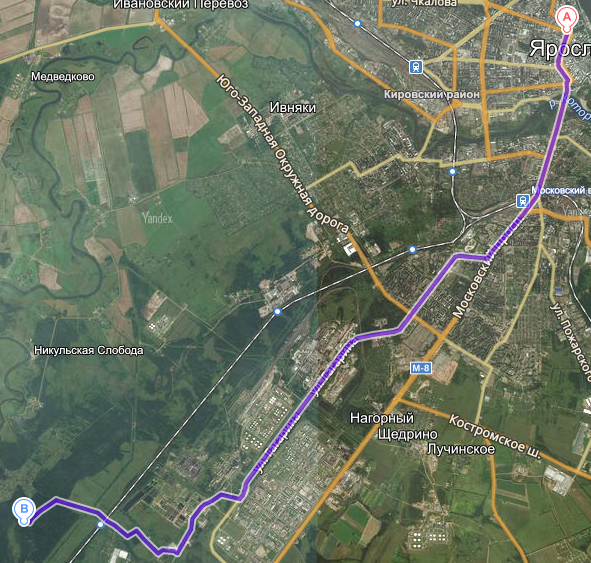
\includegraphics[width=1.0\linewidth]{YandexMap}}
	\caption{Общий вид маршрута}
	\label{ris:generalRoute}
\end{figure}

\newpage
\subsection*{Детализация проезда}
\par Первое, что Вам необходимо сделать, что бы добраться до посвята своим ходом --- добраться до улицы Гагарина. По этой улице нужно ехать до проходных НПЗ. НИКУДА НЕ СВОРАЧИВАТЬ! Даже если Вы и Ваша спутница в один голос орете, что узнаете место и нужно ехать направо. НЕТ! До проходных НПЗ. Там есть остановки автобусов и круговое движение (см. рисунок~\ref{ris:NPZ}).

\begin{figure}[h]
	\center{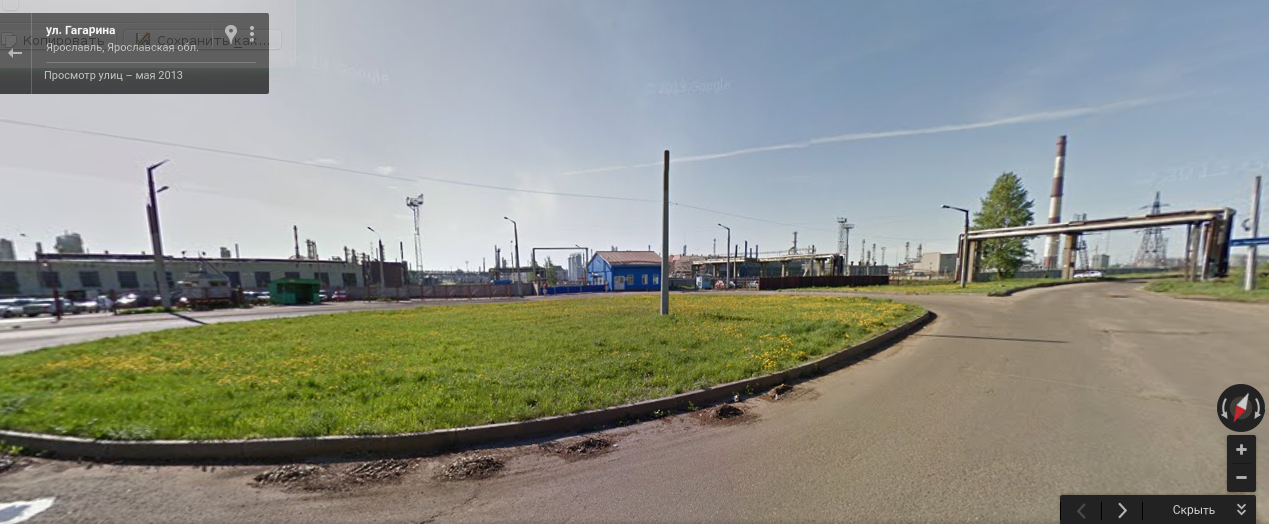
\includegraphics[width=1.0\linewidth]{NPZ}}
	\caption{Проходные НПЗ}
	\label{ris:NPZ}
\end{figure}

\par Затем нужно продолжить движение по улице Гагарина и повернуть направо, на самом деле правильнее сказать <<продолжить движение по улице Гагарина>>, так как она по факту поворачивает направо (см. рисунок~\ref{ris:afterNPZ}).

\begin{figure}[h]
	\center{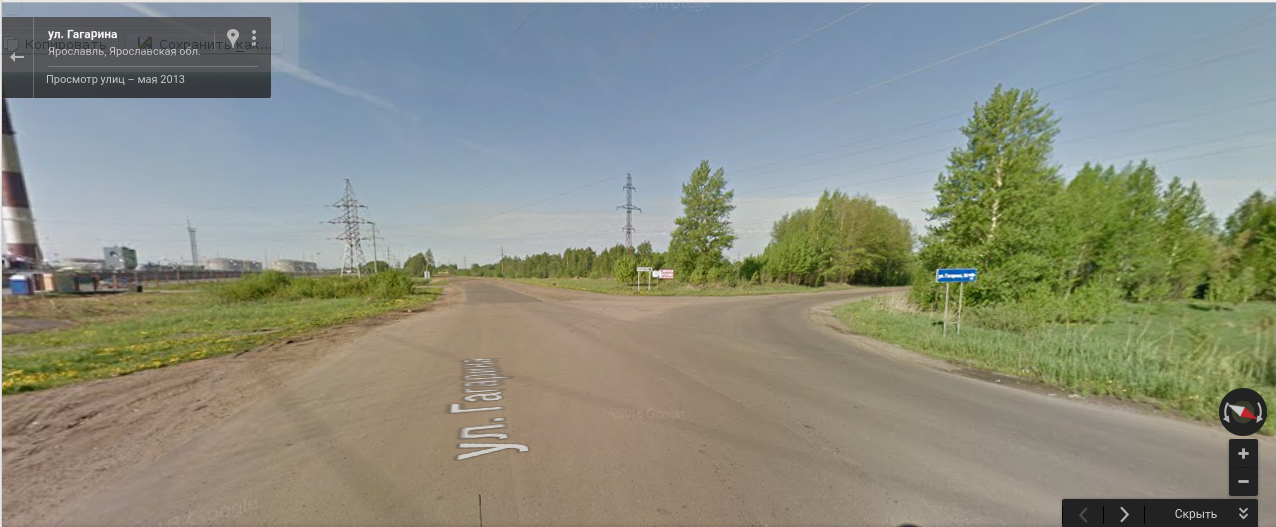
\includegraphics[width=1.0\linewidth]{afterNPZ}}
	\caption{Поворот после проходных}
	\label{ris:afterNPZ}
\end{figure}

\par Теперь начинается самое веселое. Нужно ехать по этому подобию дороги и никуда не сворачивать. Я понимаю, что это звучит глупо, но Вы все еще едете по улице Гагарина. Необходимо добраться до забора (см. рисунок~\ref{ris:zabor}) и повернуть направо. Ехать вдоль него. Дорога там одна. Доезжаете до жд переезда и можете считать, что удачно добрались. Не проспите последний поворот налево (см. рисунок~\ref{ris:last}).

\begin{figure}[h]
	\center{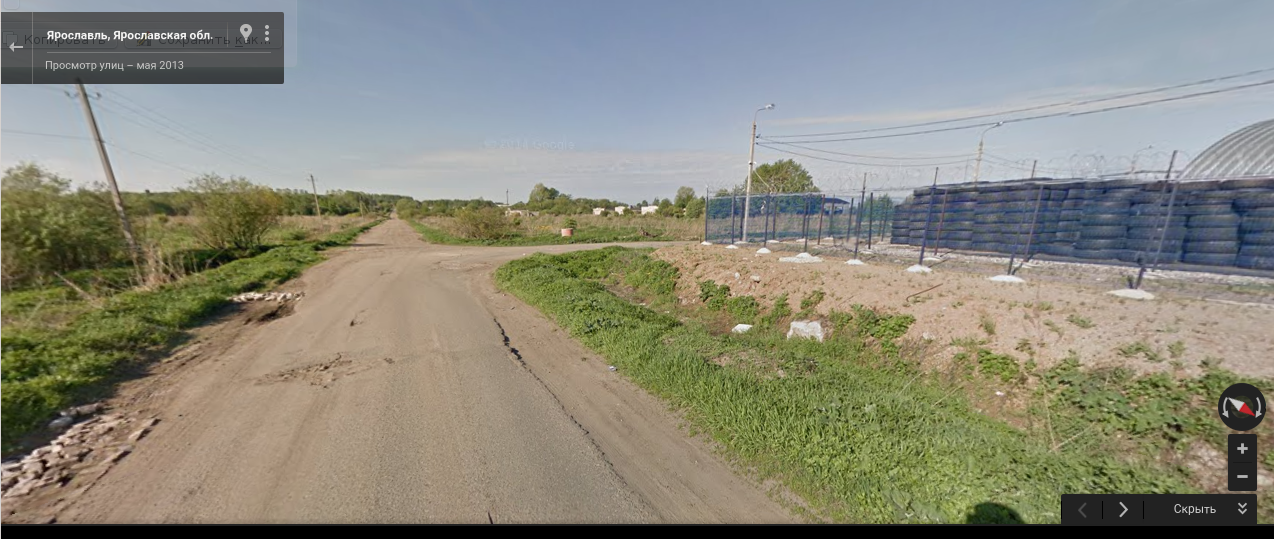
\includegraphics[width=1.0\linewidth]{zabor}}
	\caption{Забор}
	\label{ris:zabor}
\end{figure}

\begin{figure}[h]
	\center{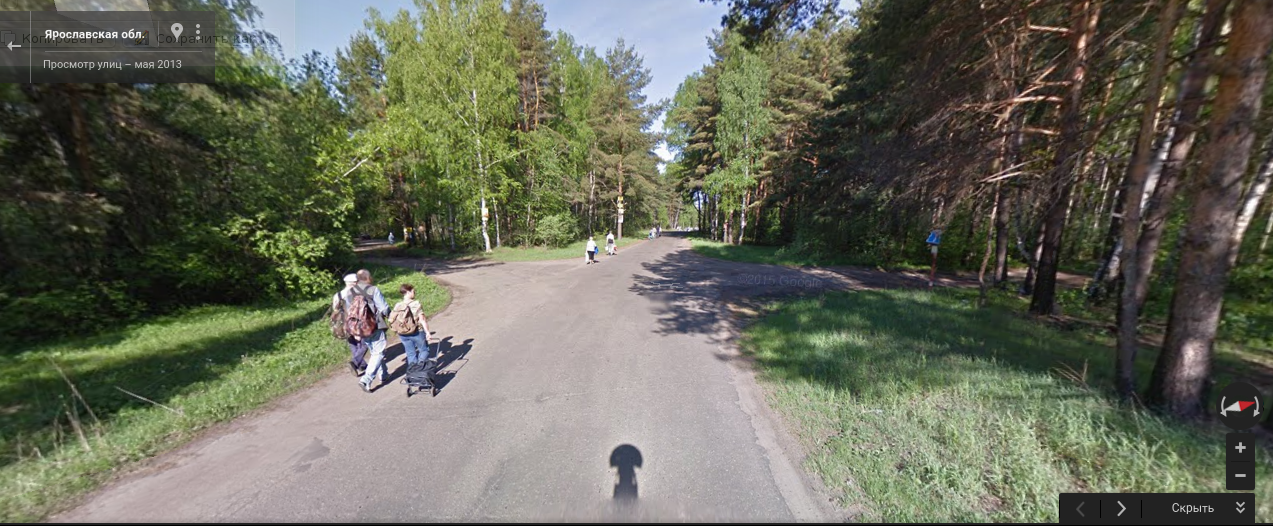
\includegraphics[width=1.0\linewidth]{last}}
	\caption{Посвят близок}
	\label{ris:last}
\end{figure}

\end{document}